\documentclass[../5RO17_TP1.tex]{subfiles}

\begin{document}
\subsection{Question 4}

Le fichier \textit{q1.py}, associé à la bibliothèque de fonctions \textit{q1\_lib.py}, contient le code avec les modifications nécessaires pour réaliser le panorama. Différentes techniques, en plus de la simple homographie avec des points communs arbitraires, ont été utilisées pour obtenir des résultats plus intéressants, comme le choix stratégique des points, la correction de couleur et l'application d'un filtre gaussien dans les régions superposées. Ces développements sont expliqués ci-dessous.

\subsubsection{Homographie}

La première idée pour la construction du panorama était de réaliser une homographie sur les images latérales en utilisant des correspondances arbitraires de points. Nous avons pris soin de translater les images de manière à ce que ces points se superposent. Bien qu'il ait été possible d'obtenir un résultat visuellement continu, certaines combinaisons de points sélectionnés créaient des trous près des coins des images, entraînant une visualisation peu agréable pour un panorama, comme le montre l'exemple ci-dessous.

% fig ici
\begin{figure}[h]
    \centering
    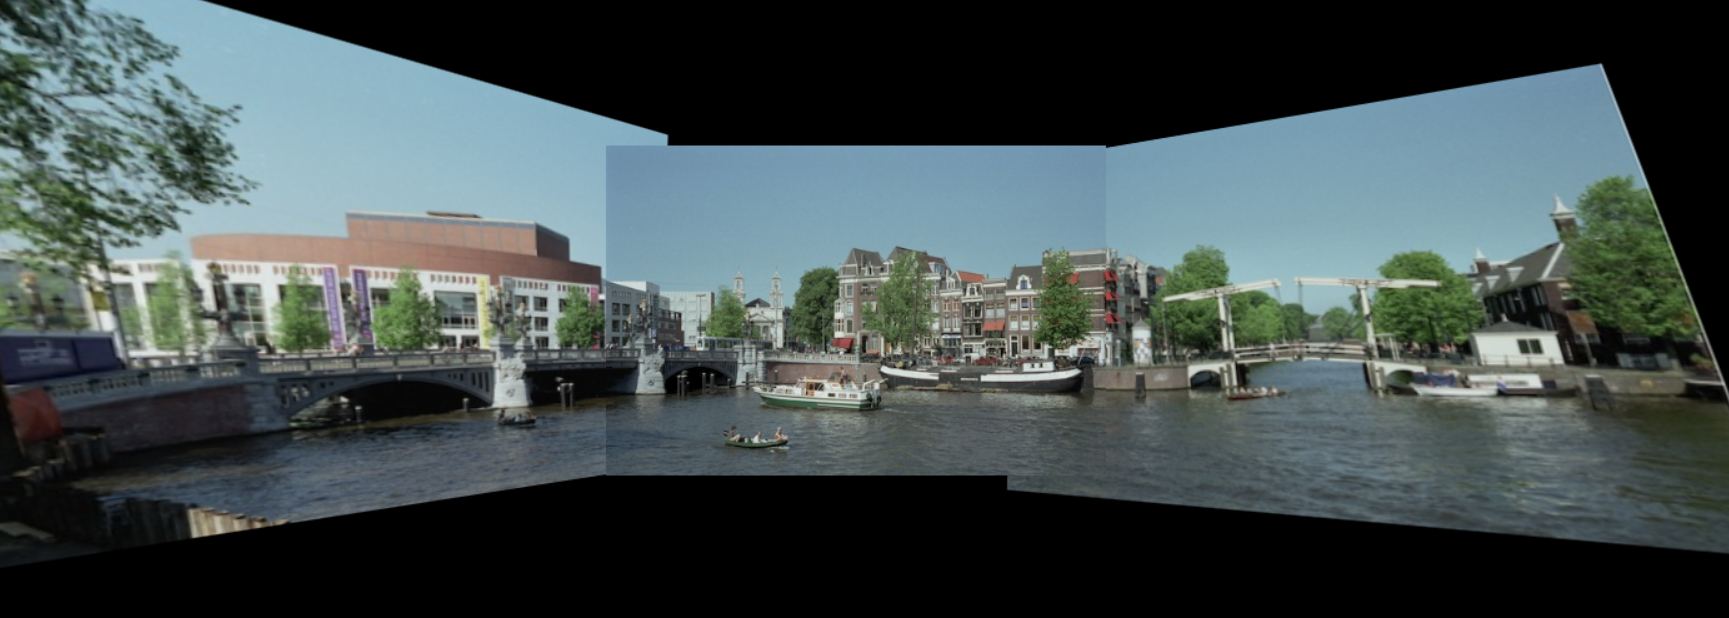
\includegraphics[width=0.6\linewidth]{images/amsterdam_0.png}
    \caption{Résultat sans traitement.}
    \label{fig:ams0}
\end{figure}

Pour résoudre ce problème, la première solution envisagée consistait à mieux sélectionner les points correspondants afin de mieux aligner les coins des images et d'éviter ces zones noires. Pour cela, nous avons ajouté des points supplémentaires sur les bords supérieur et inférieur (à la même position en y que le point le plus proche du bord) aux points utilisés pour le calcul de l'homographie. Voici le code correspondant :

\begin{scriptsize}\mycode
	\begin{lstlisting}[language=Python]
# Add boundary points for alignment
X_init1.append([max([point[0] for point in X_init1]), new_height - 1])
X_init1.append([max([point[0] for point in X_init1]), 0])
X_final2.append([min([point[0] for point in X_final2]), new_height - 1])
X_final2.append([min([point[0] for point in X_final2]), 0])
X_final1.append([max([point[0] for point in X_final1]), new_height - 1])
X_final1.append([max([point[0] for point in X_final1]), 0])
X_init2.append([min([point[0] for point in X_init2]), new_height - 1])
X_init2.append([min([point[0] for point in X_init2]), 0])
	\end{lstlisting}
\end{scriptsize}

En général, cette approche a conduit à des résultats plus satisfaisants, comme le montre la figure \ref{fig:ams1} suivante.

\begin{figure}[!h]
    \centering
    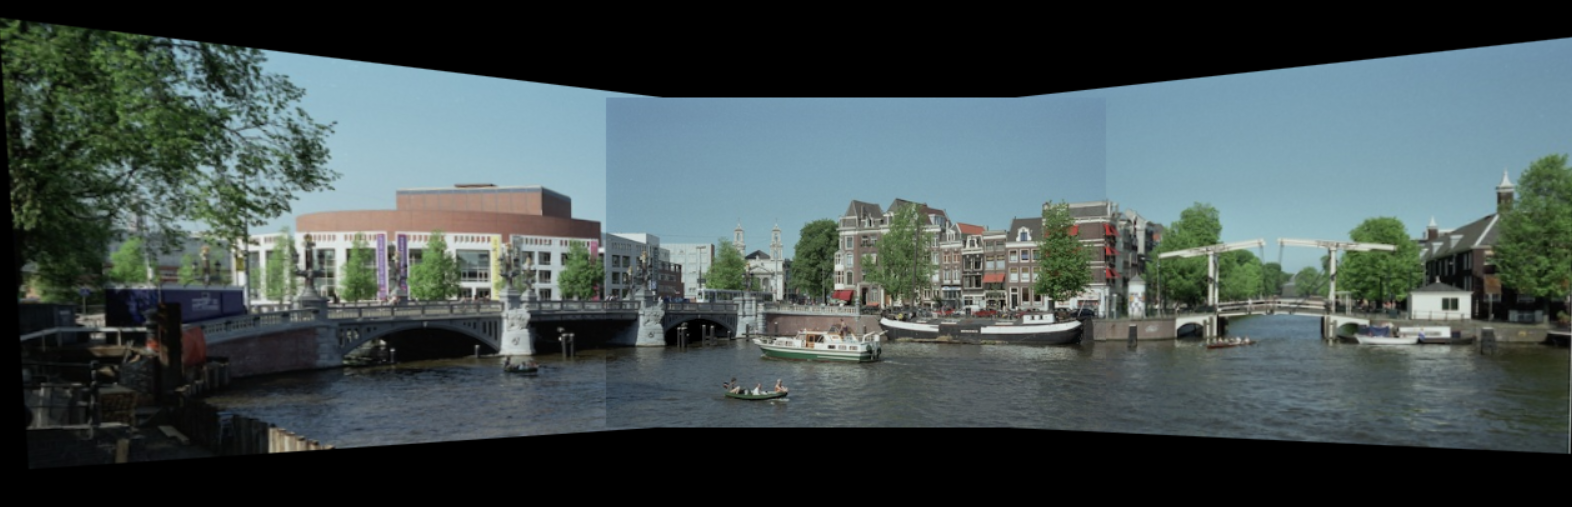
\includegraphics[width=0.6\linewidth]{images/amsterdam_sans_color.png}
    \caption{Résultat avec une choix stratégique des points.}
    \label{fig:ams1}
\end{figure}

% fig ici

Cependant, une discontinuité importante persistait dans les transitions entre les images, nécessitant d'autres ajustements.
\subsubsection{Correction de couleurs}

Une première idée pour résoudre cette différence observée a été de réaliser un traitement de couleur afin d'égaliser les tonalités entre les deux images. Pour cela, nous avons choisi un point dans chaque image (le premier à être sélectionné pour l'homographie) qui devrait avoir la même couleur. Idéalement, ce point se trouve sur une surface uniforme, comme le ciel dans cette image d'Amsterdam, afin d'obtenir de bons résultats. Ensuite, nous avons appliqué à toute l'image latérale la différence de couleur entre ces points pour les égaliser. Voici le code correspondant :

\begin{scriptsize}\mycode
	\begin{lstlisting}[language=Python]
def fix_color(img_source, img_reference, x_source, y_source, x_ref, y_ref):

    # Get pixel colors for color adjustment
    color_source = img_source[y_source, x_source].astype(np.float32)
    color_reference = img_reference[y_ref, x_ref].astype(np.float32)

    # Calculate the necessary color adjustments and applies
    diff = color_reference - color_source
    img_source = cv2.add(img_source.astype(np.float32), diff)

    # Clip pixel values to valid range
    img_source = np.clip(img_source, 0, 255).astype(np.uint8)

    return img_source

# Apply color adjustments to images
img1 = fix_color(img1, img2, int(X_init1[0, 0]), int(X_init1[0, 1]), int(X_final1[0, 0]), int(X_final1[0, 1]))
img3 = fix_color(img3, img2, int(X_init2[0, 0]), int(X_init2[0, 1]), int(X_final2[0, 0]), int(X_final2[0, 1]))
	\end{lstlisting}
\end{scriptsize}

Cette approche a considérablement amélioré les transitions entre les images, comme on peut le voir dans la Figure \ref{fig:ams2}. La petite disparité restante a été résolue en appliquant un filtre pour adoucir le gradient.

\begin{figure}[h]
    \centering
    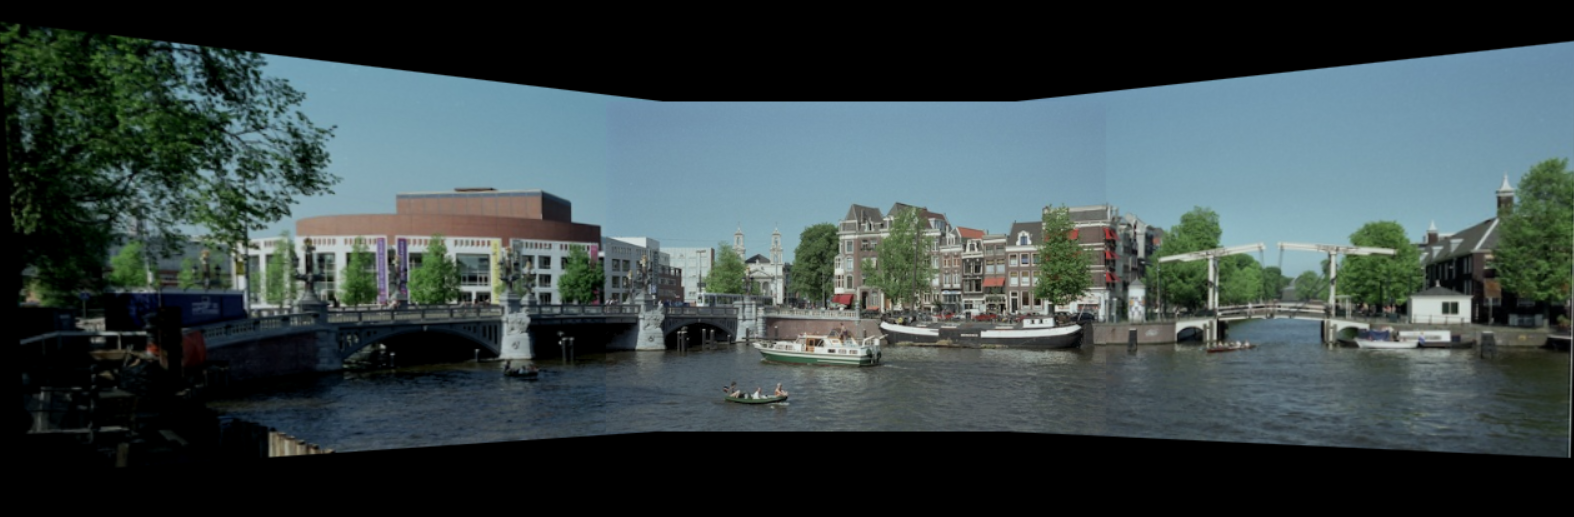
\includegraphics[width=1\linewidth]{images/amsterdam_sans_blend.png}
    \caption{Résultat l'égalisation de coleurs.}
    \label{fig:ams2}
\end{figure}


\subsubsection{Filtre de fusion progressive}

Enfin, pour résoudre les artefacts de division restants, un filtre en dégradé a été ajouté pour assurer une transition plus fluide dans les régions superposées, comme illustré dans l'extrait de code ci-dessous :

\begin{scriptsize}\mycode
	\begin{lstlisting}[language=Python]
    ...

    # Blend img1 and img2 in the left overlap region
    elif left_blend_start <= col < left_blend_start + blend_region_width:
        blend_position = col - left_blend_start
        alpha = blend_position / blend_region_width
        img2[row, col] = (1 - alpha) * img1_warp[row, col] + alpha * img2[row, col]

    # Blend img2 and img3 in the right overlap region
    elif right_blend_end - blend_region_width <= col < right_blend_end:
        blend_position = col - (right_blend_end - blend_region_width)
        alpha = blend_position / blend_region_width
        img2[row, col] = (1 - alpha) * img2[row, col] + alpha * img3_warp[row, col]
	\end{lstlisting}
\end{scriptsize}

Ce filtre de fusion progressive permet de rendre la transition entre les images plus homogène dans les zones de chevauchement, en utilisant un coefficient \(\alpha\) qui varie linéairement en fonction de la position dans la région de superposition. Cela permet de réduire les discontinuités visibles et de créer un rendu plus cohérent dans la composition finale. 

\begin{figure}[h]
    \centering
    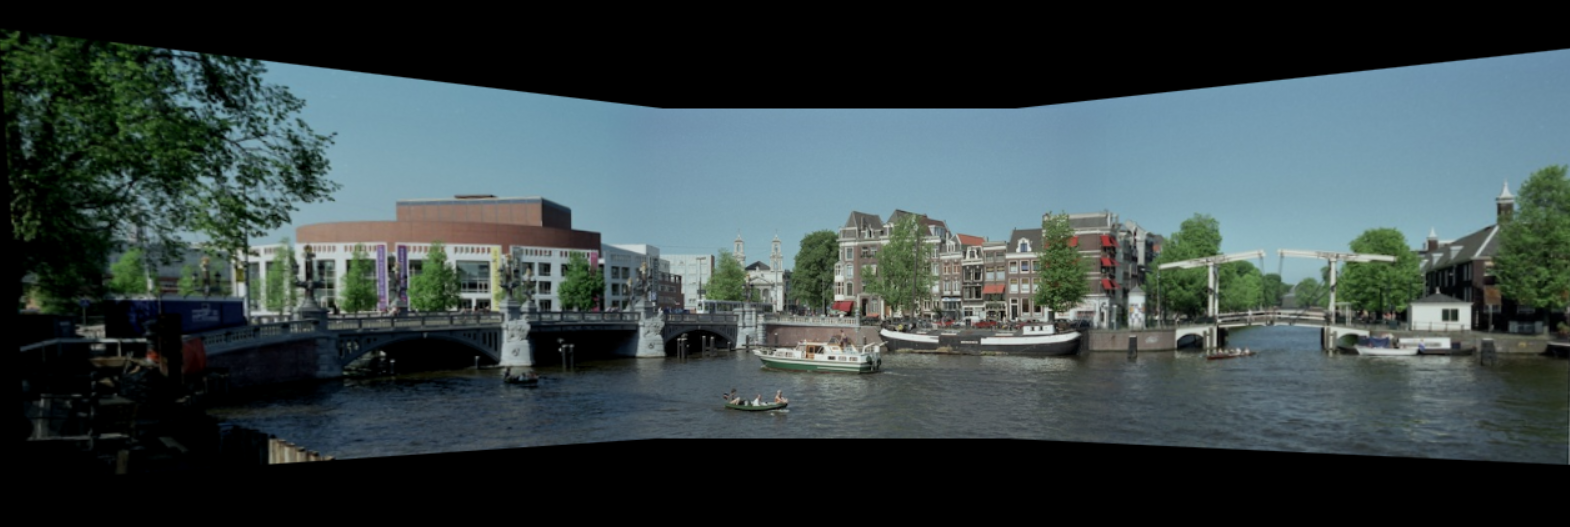
\includegraphics[width=1\linewidth]{images/amsterdam_final.png}
    \caption{Résultat final.}
    \label{fig:ams3}
\end{figure}

Les mêmes résultats présentés dans ce rapport pour les autres images exemples peuvent être obtenus en exécutant le code avec la flag \textit{USE\_PRE\_SELECTED\_POINTS} égale à \textit{True}.

\subsection{Questions}

1. \textbf{Quelle condition doit respecter la prise de vue entre les deux images?}

Pour réaliser l'homographie entre deux images, il est essentiel que ces dernières possèdent un recouvrement suffisant. Cela permet de détecter des points d'intérêt communs. De plus, la différence de point de vue entre les deux images doit être essentiellement une simple rotation. En effet, c'est uniquement dans ce cas que la transformation de l'image projetée peut être décrite par une homographie, et elles représentent alors une bonne approximation du point de vue central élargi.

\medskip

2. \textbf{Comment retrouver les paramètres de cette transformation à partir de ceux de l’homographie?}

Comme indiqué dans le matériel de cours, pour une rotation simple, il est possible de réécrire la transformation sous la forme :

\[
\tilde{m}' = K R K^{-1} \tilde{m}
\]

Dans ce contexte, l'homographie, qui est connue, est égale à \( K R K^{-1} \), où \( R \) contient les informations sur la rotation réalisée, et \( K \) représente les paramètres intrinsèques de la caméra. Par conséquent, si nous connaissons les caractéristiques de la caméra utilisée, nous pouvons retrouver \( R \) et ainsi obtenir les paramètres de la rotation observée.




\end{document}
